When we are calculating the Assymetric Shapley Value we need a casualty DAG $G$ that defines the relationship between the features and a probability distribution $Pr$ function. In our case we will be using Bayesian Networks as $G$ and $Pr$, it will define the probability of each feature and also the casualty graph. A Bayesian Network $B$ is a $DAG$, where each node represents a different variable and the arcs represent the conditional dependencies between them. For example, if we have the arc $A \longrightarrow B$ then this represents that the variable $B$ is dependent on $A$, and that is quantified using the conditional probability $P(B|A)$. A node can have multiple parent's, so the probability of the node will be defined in a \emph{Conditional Probability Table} (CPT), the probability of the node taking on a particular value, given the values of its parent node. With that, we can define a Bayesian Network as:

\begin{definition}
A Bayesian Network consists of the following:

\begin{itemize}
    \item A set of variables and a set of directed edges between variables, where each variable has a finite set of mutually exclusive states.
    \item The variables together with the directed edges form an acyclic directed graph (traditionally abbreviated DAG); a directed graph is acyclic if there is no directed path $A_1 \rightarrow \dots \rightarrow A_n$ so that $A_1 = A_n$.
    \item To each variable $A$ with parents $B_1, \dots, B_n$, a conditional probability table (CPT) $P(A \mid B_1, \dots, B_n)$ is attached.
\end{itemize}
    
\end{definition}

\begin{figure}[ht]
    \centering
    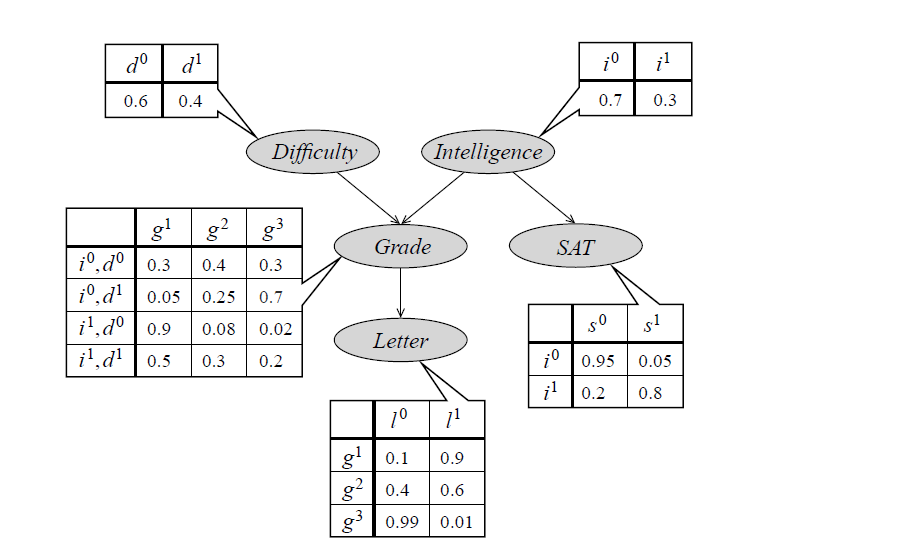
\includegraphics[scale=0.4]{img/bayesianNetworks.png}
    \caption{Bayesian Network for determining a students' intelligence. We can see that each node has a $CPT$ that it's calculated based on it's parent's, here the variables are binary.}
    \label{fig:bayesian_network_example}
\end{figure}

\newpage
 
 This kind of networks help us to simplify the computation of joint probability distributions. One of its most important properties, it's the \emph{chain rule}, it provides a  fundamental structure for understanding how joint probabilities can be decomposed in the context of Bayesian networks. Specifically, it states that if we let \( BN \) be a Bayesian network over a set of variables \( \{A_1, \dots, A_n\} \), then \( BN \) specifies a unique joint probability distribution \( P(U) \), where \( U = \{A_1, \dots, A_n\} \), that can be expressed as the product of all CPT's specified in \( BN \). Mathematically, it is represented as:
\[
P(U) = \prod_{i=1}^{n} P(A_i \mid \text{pa}(A_i))
\]
where \( \text{pa}(A_i) \) denotes the parents of \( A_i \) in the Bayesian network. This rule is essential because it simplifies the computation of the joint probability distribution of a complex network by breaking it down into simpler, local dependencies between a node and its direct predecessors. Thus, the chain rule encapsulates the essence of Bayesian networks, where local dependencies aggregate to define a global distribution, facilitating both the learning and inference processes within these networks.

%Hablar acerca de las operaciones que se pueden hacer, inferencia e instanciar variables + sus complejidades según los tipos de redes con los que uno trabaja

Furthermore, Bayesian networks facilitate a variety of computational operations crucial for probabilistic inference. One of the primary operations is \textbf{inference}, which involves computing the prior distribution for some variable. That means, calculating $Pr(A)$, being $A$ a node in the network. This process is often referred to as \emph{querying} the network. The complexity of inference depends on the network's structure, for polytree-shaped, also known as \emph{singly connected},  networks, the complexity is polynomial on the size of the network variables. \cite{pearl1986bayesianInference}. 

Another critical operation is \textbf{variable instantiation}, which involves setting the values of certain variables and observing the effects on the probabilities of other variables. In this case, we are introducing evidence into the network, which is the posterior distribution. An algorithm that we can use to perform these operations is the \emph{Variable Elimination}.\cite{Darwiche_2009} This algorithm can also run in polynomial time for polytree-shaped networks. That means that these two operations, inference and variable instantiation, can be done in a tractable manner for polytrees. 

%Encontre una cota acá, pero no pude encontrar la fuente de donde la sacan. https://www.ime.usp.br/~ddm/courses/mac6916/varelim/#computational-complexity. La cota es O((m+n)*c^(w+1)), siendo c la cardinalidad máxima de alguna de las variables (2 en nuestro caso) y w es la "induced-width of the elimination ordering plus one.". Que en el caso de polytrees, cómo podemos elegir un orden de eliminación óptimo, w está acotado por el tree width. 

%El tree width de un polytree es igual a la máxima cantidad de padres de un nodo, por lo que acotar el grado de entrada de cada nodo nos da una cota para la treeWidth. 
%Revisar mejor de acá https://www.cs.toronto.edu/~hojjat/384f06/Lectures/Lecture17-4up.pdf

%TODO: ¿Hablar más en detalle del algoritmo, del tree-width y de cómo surge esta cota?

%https://cse.hkust.edu.hk/~lzhang/paper/pspdf/canai94.pdf Acá se introdujo el algoritmo de Variable Elimination 

\newpage

%TODO: Hablar de cómo lo nuestro solo funciona para trees actualmente entonces cómo podemos pasar nuestra red bayesiana a un decision tree. 

\begin{comment}
    Quiero remover algunos ejes de la red bayesiana para que me quede un árbol.
Heurística para ver que ejes remover:
¿El eje que me genere un ciclo + genere una menor divergencia entre las distribuciones marginalizadas?
La idea sería fijarse que distribuciones me quedan al removerlo, luego comparar cuáles son las que divergen menos entre sí (criterio KL por ejemplo) y elegir ese eje. 
\end{comment}

\subsubsection{Mean prediction in Decision Trees}

Decision Trees are widely utilized in Artificial Intelligence (AI) for their ability to make predictions and classifications based on features from input data.By breaking down decisions into a series of straightforward questions and answers, decision trees allow users to understand the reasoning behind AI predictions, contributing to transparency in complex systems.

The primary components of a decision tree include nodes, branches, and leaves. Each internal node represents a "condition" based on input features, which bifurcates the data into branches according to their answers. Leaves represent the final outcomes, providing the decision or prediction. There is a direct relationship between the tractability of the \emph{mean} of a model and the $ASV$ \santi{SV?} when the distribution is a \emph{fully factorized} one. So we wanted to see if the calculation of the mean was tractable for decision trees with Bayesian networks distributions, that's how we found this algorithm. \\

%TODO: Redactarlo mejor

For this algorithm, we are going to be working with decision trees, and the features in the tree will be binary. Each node determines a value for one feature $X_i$, with the left child being the case where $X_i=0$ and the right one. They will be a set $X$, and their probability distribution will be a Bayesian network $B$. Then $Pr_B(X_i = k)$ is the probability that the feature $i$ is $k$ given the Bayesian network $B$. And $B_{X_i=k}$ is the Bayesian network $B$ with the feature $i$ instantiated in $k$. 

%TODO: Redactar mejor lo del decision tree binario. 

%TODO: Definimos que nuestra variable a predecir no puede estar en el grafo causal, que no tiene mucho sentido nuestro algoritmo si ese es el caso. Por lo que definimos remover ese feature de nuestra red causal. Agregar esto

%TODO: Hablar de esta operación -> Implementar la operación en las redes bayesianas de <= + probar de calcular el promedio en una red más grande cómo CHILD

\begin{algorithm}
\caption{Mean for Binary Decision Tree}
\begin{algorithmic}[1]
\Function{Mean}{$node$, $B$, $pathCondition$, $evidence$}
    \If{$n$.isLeaf}
        \State \Return  $Pr_B(pathCondition\ | \ evidence)$ * $node.value$
    \EndIf
    \State $X_i \gets n.feature$
    \State $leftMean \gets$  \Call{Mean}{$node$.left, $B$, $pathCondition \cup \set{X_i=0}, evidence$}
    \State $rigthMean \gets$ \Call{Mean}{$node$.right, $B$, $pathCondition \cup \set{X_i=1}, evidence$} 
    \State \Return  \mbox{$leftMean + rigthMean$}
\EndFunction
\end{algorithmic}
\end{algorithm}

Let's analyze the complexity of this algorithm. The operation $Pr_B(X_i = k | evidence)$ is the inference in a Bayesian Network, that means that it has  polynomial time complexity. That implies that the cost of processing each node is polynomial, so the runtime complexity of this algorithm will be polynomial in the size of the decision tree and the Bayesian network. 

%¿Polinomial en base a que? ¿Aclaro de vuelta todo lo anterior? Siento que estoy diciendo todo el tiempo lo mismo, necesito sinonimos de polinomial. ¿Lo hago más formal?

\begin{figure}[ht]
    \centering
    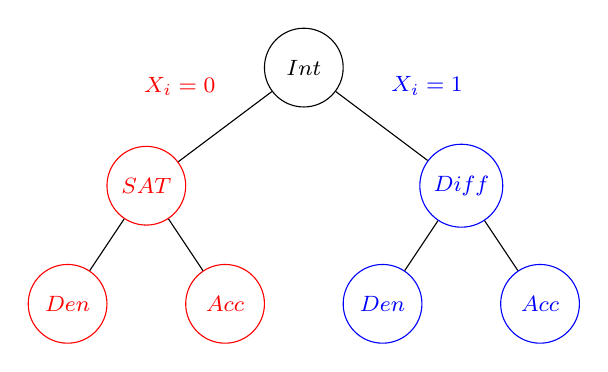
\begin{tikzpicture}[
    level 1/.style={sibling distance=4cm},
    level 2/.style={sibling distance=2cm},
     every node/.style={minimum size=1cm, font=\footnotesize} % Adjust size as needed
]
    \node [circle, draw] {$Int$}
        child {node [circle, draw, red] {$SAT$}
            child {node [circle, draw, red] {$Den$}}
            child {node [circle, draw, red] {$Acc$}}
            edge from parent node[above left] {\textcolor{red}{$X_i=0$}}
        }
        child {node [circle, draw, blue] {$Diff$}
            child {node [circle, draw, blue] {$Den$}}
            child {node [circle, draw, blue] {$Acc$}}
            edge from parent node[above right] {\textcolor{blue}{$X_i=1$}}
        };
    \end{tikzpicture}
    
    \caption{Decision tree for determining if a student will be accepted or denied into a university based on the features of the Bayesian network of figure \ref{fig:bayesian_network_example}.}
    \label{fig:decision_tree_example}
\end{figure}

In figure \ref{fig:decision_tree_example} we have an example of a decision tree. If we run this in the root node of the tree, we will obtain: \echu{Esto ahora no tiene sentido, debería cambiar las cuentas en base a la nueva fórmula}
\begin{align*}
        \Call{Mean}{Int, B} &= Pr_B(Int = 0) * \Call{Mean}{SAT, B_{Int=0}} + Pr_B(Int = 1) * \Call{Mean}{Diff, B_{Int=1}}\\
        &= 0.7 * \Call{Mean}{SAT, B_{Int=0}} +0.3 * \Call{Mean}{Diff, B_{Int=1}} \\
        &= \dots \\
        &= 0.234
    \end{align*}

% Estas cuentas son números cualquiera, tengo que hacerlas y reemplazar con el resultado correcto. 
and we can keep doing this to obtain the result \textbf{calcular el promedio, je}. 

\subsubsection{Time complexity of mean prediction in DT}
% Here we want to compare the naive way (obtaining all the consistent instances vs the mean prediction). 
% We can also compare the time it takes for both and the improvement that the algorithm has versus the naive way. 

\subsubsection{Exact mean prediction computation in Decomposable Circuits}

Can we extend the previous algorithm to work in more general models? We can easily prove an upper bound on model complexity related to the satisfiability problem.

\begin{proposition}
    Let $M$ be a model over entities $\entities(X)$ and $\aDistribution$ a distribution over $\entities(X)$ such that no entity has probability 0. Then, deciding if $\expectancy_{e\sim \aDistribution}[M(e)]$ is positive is equivalent to deciding if $M$ is satisfiable.
\end{proposition}

This does not rule out the tractability of exactly computing the average of models for which the satisfiabilily problem is tractable, such as d-DNNF circuits \cite{arenas2021tractability}. For them, we can prove an intractability result exploiting the correlations that one can impose using the Bayesian Network, which allows us to turn a normal Boolean circuit into a d-DNNF one without altering the average prediction.

\begin{proposition}
    The problem of deciding, given a Bayesian distribution $\aBayesianDistribution$ and a d-DNNF circuit $\aCircuit$ whether $\expectancy_{e \sim \aBayesianDistribution}[\aCircuit(e)] > 0$ is \NPhard{}. Moreover, the results holds for Bayesian Networks which are union of disjoint paths.
\end{proposition}

\begin{proof}
    The problem clearly belongs to $\NP{}$, since we can solve it by guessing an entity $e$ such that $\aCircuit(e)$ and $\Pr[e] > 0$. For the hardness, we reduce \textsc{Circuit-SAT} to our problem.

    Let $\aCircuit$ be a Boolean circuit. Without loss of generality we may assume that it is deterministic (i.e. for each $\vee$ gate the two subcircuits $\aCircuit_1$ and $\aCircuit_2$ cannot be simultaneously satisfied). We are going to design a simple Bayesian distribution such that $\aCircuit$ can be understood also as a decomposable circuit.

    We proceed top-down. Let $\wedge$ be the \textit{and} node closest to the top, and let $\aCircuit_1$ and $\aCircuit_2$ the two subcircuits of this node. In principle, $var(\aCircuit_1) \cap var(\aCircuit_2) \neq \emptyset$. To fix this, let $x_1,\ldots, x_k$ be the variables shared by both subcircuits, and replace the variables $x_1,\ldots,x_k$ from $\aCircuit_2$ with the variables $x_1',\ldots,x_k'$. At the same time, we add to the Bayesian network nodes $x_1,x_1',\ldots,x_k,x_k'$ conditioning that whenever $x_i = 1$ then $x_i'=1$ with probability one, and similarly for the case $x_i = 0$, for all $i$.

    Observe that some entities have probability 0: they are exactly those that pick a different value for $x_i$ and $x_i'$, for some $i$. Therefore, if the expected value of this new circuit is positive then there is an assignment of the original circuit such that it is satisfied.

    To complete the reduction we continue working recursively: at each $\wedge$ gate we detect the shared variables $y_1,\ldots,y_\ell$, change them with variables $y_1',\ldots,y_\ell'$ and add the correlations in the Bayesian network $\aBayesianDistribution$.

    Note that the final structure of the Bayesian network is a set of disjoint paths, over which the inference problem be solved easily.
\end{proof}

\subsection{Approximate mean prediction computation}

Even though exact computation is intractable, approximate calculation is straightforward when considering additive precission.

\begin{proposition}
    Let $\aDistribution$ be any distribution over $\entities(X)$ that can be sampled efficiently, and $\mathcal{F}$ a family of models such that evaluating, given $M \in \mathcal{F}$ and $e \in \entities(X)$, the value $M(e)$,q can be done in polynomial time. Then, there is a \textit{Fully Polynomial-time Approximation Scheme} (FPRAS) for $\expectancy_{e \in \aDistribution}[M(e)]$ under additive error\footnote{I don't think we can achieve multiplicative error, looks like satisfiability.}.
\end{proposition}

\begin{proof}
    Note that $M(e) : \aDistribution \to \{0,1\}$ is a random variable bounded between $0$ and $1$ that can be sampled efficiently, and thus the result follows by considering the Hoeffding's inequality.
\end{proof}


%Tiene sentido poner que no se puede? Y la demo esa de convertir una red no deterministica en una deterministica en polinomial? O alguna otra justificación?